\section{Zielsetzung und Anforderungen}

Ziel dieses Kapitels ist die Darstellung der technischen Anforderungen und der strukturellen Umsetzung der entwickelten Platine. Die Schaltung dient als Demonstrations- und Lehrgerät zur Veranschaulichung synthetisch erzeugter EEG-Signale im schulischen oder hochschulischen Unterricht.
Kernziel der Platine ist die Erzeugung und analoge Ausgabe von EEG-Signalen über vier getrennte Kanäle. Die Parametrierung der Signale erfolgt über eine browserbasierte Benutzeroberfläche, die ohne zusätzliche Softwareinstallation genutzt werden kann. Die gesamte Steuerung und Ausgabe wird durch einen Mikrocontroller übernommen, der sowohl die Signalverarbeitung als auch die Bereitstellung der Weboberfläche realisiert.
Zur Sicherstellung einer realistischen Signalform und zur Rauschunterdrückung kommen ein hochauflösender Digital-Analog-Wandler sowie nachgeschaltete analoge Tiefpassfilter zum Einsatz. Zusätzlich wird das Ausgangssignal über einen Spannungsteiler skaliert, um typische EEG-Signalpegel im Mikrovoltbereich darzustellen.
Die folgenden Abschnitte beschreiben die eingesetzten Komponenten, ihre Auswahlkriterien und die Umsetzung auf der entwickelten Platine.


\chapter{Platine}

\section{Komponentenübersicht}

Für die Umsetzung der Platine wurden gezielt Bauteile ausgewählt, die eine zuverlässige Signalverarbeitung sowie eine einfache Integration in ein schulisches Umfeld ermöglichen. Die wichtigsten Hardwarekomponenten sind:

\begin{itemize}
  \item \textbf{Mikrocontroller:} ESP32-S3 16R8 – steuert die gesamte Signalverarbeitung, erzeugt die digitalen Datenmuster und stellt die Weboberfläche über WLAN bereit.
  \item \textbf{Digital-Analog-Wandler (DAC):} DAC8412FPZ – ermöglicht die hochauflösende, analoge Ausgabe der zuvor digital berechneten EEG-Signale auf vier unabhängigen Kanälen.
  \item \textbf{Operationsverstärker:} TL071CDR – dient als aktiver Tiefpassfilter (1. Ordnung) mit einer Verstärkung von 1 zur Glättung der analogen Ausgangssignale.
  \item \textbf{Spannungsversorgung:}
  \begin{itemize}
    \item \textbf{NCV1117DT50:} Linearregler zur Bereitstellung einer stabilisierten 5-V-Spannung für den DAC und nachgeschaltete Stufen.
    \item \textbf{USB-C-Buchse:} Dient sowohl der Stromversorgung als auch der optionalen Datenverbindung während der Entwicklung.
  \end{itemize}
\end{itemize}


\subsection{Hardwarekonzept}

Der Mikrocontroller ESP32-S3 16R8 bildet das zentrale Steuerelement der Platine. Er verfügt über zwei Prozessorkerne, wodurch sich die Verarbeitung von Signalmustern und die Bereitstellung der Weboberfläche auf getrennte Kerne verteilen lassen. Mit 16\,MB integriertem Flash-Speicher bietet er zudem ausreichend Kapazität zur Ablage von Firmware, Webdateien und Nutzdaten.

Für die analoge Signalausgabe wird der Digital-Analog-Wandler DAC8412FPZ von Analog Devices eingesetzt. Dieser 12-Bit-DAC besitzt vier voneinander unabhängige Ausgänge und wird über eine parallele 16-Bit-Schnittstelle angesteuert. Die Ansteuerung ermöglicht eine hohe Datenrate und unterstützt somit eine nahezu echtzeitfähige Signalübertragung.

Zur Nachbearbeitung der DAC-Ausgabe wird ein aktiver Tiefpassfilter auf Basis des Operationsverstärkers TL071CDR verwendet. Dieser glättet die Treppenspannung des DACs und unterdrückt hochfrequentes Rauschen, um ein möglichst sauberes analoges Ausgangssignal zu erzeugen.

Die Spannungsversorgung der Komponenten wird durch mehrere Regler bereitgestellt: Ein Linearregler (LDO) liefert 5\,V für den DAC und nachgeschaltete Stufen, ein weiterer LDO stellt 3{,}3\,V für den Mikrocontroller bereit. Zusätzlich erzeugt ein invertierender DC/DC-Wandler die negative Versorgungsspannung, sodass der DAC und die Operationsverstärker symmetrisch mit \(\pm5\,\text{V}\) betrieben werden können.


\section{Schaltungsdesign}
\subsection{Gesamtüberblick}
\begin{figure}[H]
    \centering
    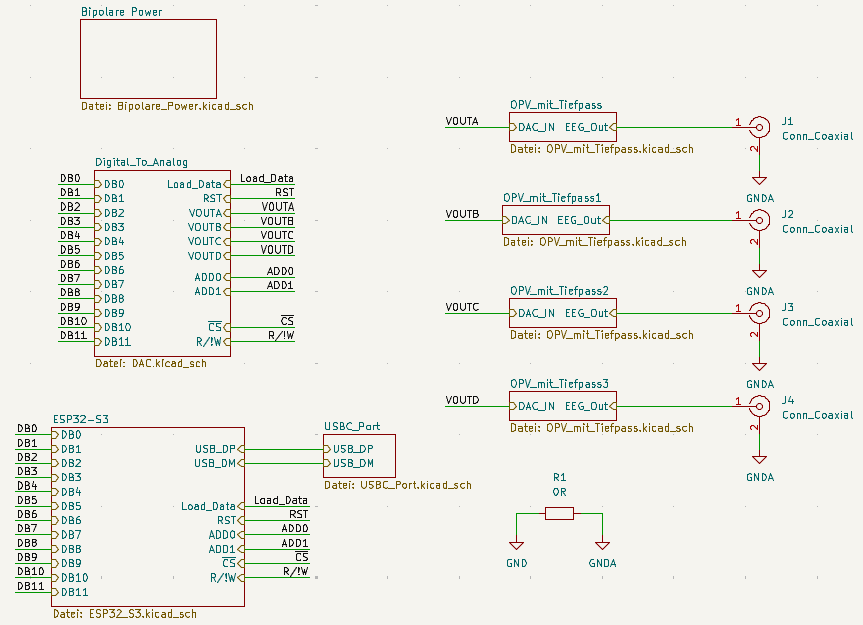
\includegraphics[width=0.8\textwidth]{bilder/Platine_gesamt.png}
    \caption{Gesamtübersicht der Platine}
    \label{fig:gesamtuebersicht}
\end{figure}
Die Schaltung ist modular aufgebaut und in mehrere funktionale Blöcke gegliedert, die jeweils klar definierte Aufgabenbereiche abdecken:

\begin{itemize}
    \item \textbf{Mikrocontroller-Block:} Beinhaltet den ESP32-S3 16R8, der die gesamte Steuerlogik sowie die Webschnittstelle übernimmt.
    \item \textbf{DAC-Block:} Umfasst den DAC8412FPZ zur Umwandlung der digitalen Signalmuster in analoge Ausgangssignale.
    \item \textbf{Operationsverstärker-Block:} Realisiert die analoge Filterung der DAC-Ausgänge mittels aktiver Tiefpassfilter.
    \item \textbf{Spannungsversorgungsblock:} Stellt alle benötigten Spannungen bereit (5 V, ±5 V, 3{,}3 V) inklusive Referenzspannungen.
    \item \textbf{USB-Block:} Dient als Schnittstelle zur Stromversorgung über USB-C.
\end{itemize}




\subsection{Mikrocontroller-Block}
\begin{figure}[H]
    \centering
    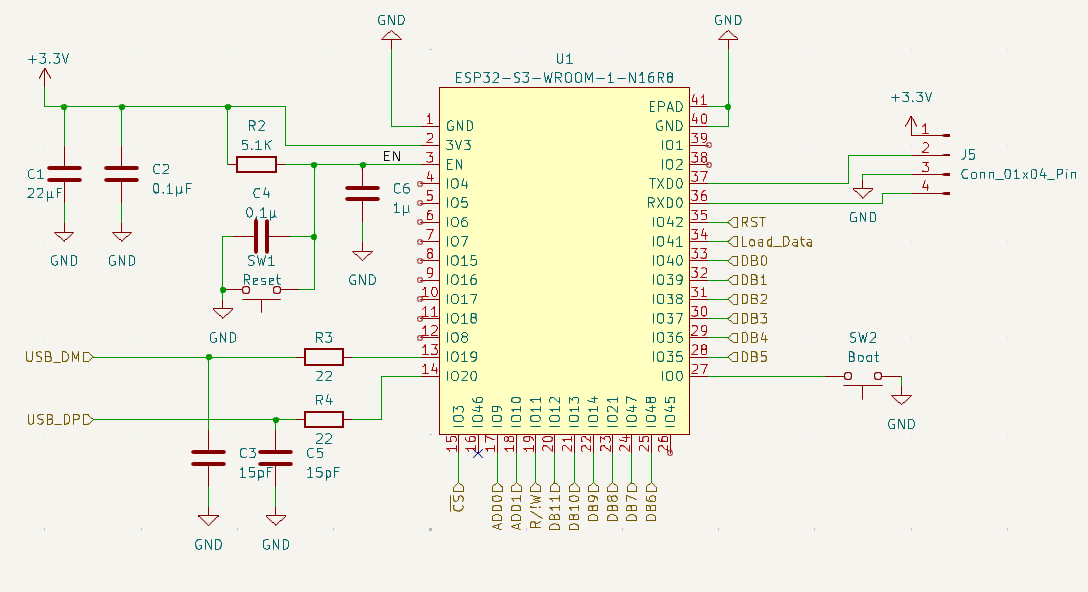
\includegraphics[width=0.8\textwidth]{bilder/Mikrocontroller_Block.png}
    \caption{Mikrocontroller-Block der Platine}
    \label{fig:mikrocontroller_block}
\end{figure}

Der Mikrocontroller-Block bildet die zentrale Steuereinheit der Platine. Herzstück ist der ESP32-S3 16R8, der sowohl die Erzeugung der digitalen EEG-Signalmuster als auch die Bereitstellung der Weboberfläche übernimmt. Die Kommunikation mit dem DAC erfolgt über eine 16-Bit-Parallelschnittstelle, wodurch eine hohe Übertragungsrate und geringe Latenz erreicht werden.
Die Programmierung des Mikrocontrollers erfolgt in C++ unter Verwendung der Arduino-Entwicklungsumgebung, ergänzt durch das Build-System PlatformIO. Neben der Echtzeitsteuerung der Signalausgabe ist der ESP32 auch für das Dateihandling sowie die Konfigurationslogik zuständig.

\subsection{DAC-Block}
\begin{figure}[H]
    \centering
    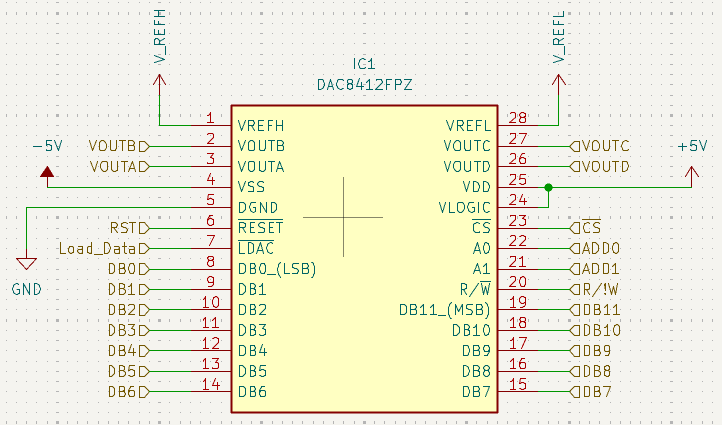
\includegraphics[width=0.8\textwidth]{bilder/DAC.png}
    \caption{DAC-Block der Platine}
    \label{fig:dac_block}
\end{figure}

Der DAC-Block umfasst den Digital-Analog-Wandler DAC8412FPZ von Analog Devices. Dieser 12-Bit-DAC ist für die Umwandlung der vom Mikrocontroller erzeugten digitalen Signalmuster in analoge Spannungen verantwortlich. 
Die Ansteuerung erfolgt über eine parallele 16-Bit-Schnittstelle, bei der alle relevanten Datenbits gleichzeitig übertragen werden. Diese Übertragungsart ermöglicht eine hohe Datentransferrate bei gleichzeitig geringer Latenz und eignet sich daher besonders für zeitkritische Anwendungen wie die synchrone Ausgabe mehrerer Kanäle.
Der DAC8412FPZ stellt vier voneinander unabhängige Ausgänge bereit. Jeder dieser Kanäle kann ein separates, kontinuierliches EEG-Signal ausgeben. Die Zuordnung der Signaldaten zu den Ausgängen erfolgt über die Softwarelogik im Mikrocontroller. Die resultierenden Spannungen an den DAC-Ausgängen werden anschließend in den analogen Nachbearbeitungsblock überführt.


\subsection{Operationsverstärker-Block}

\begin{figure}[H]
    \centering
    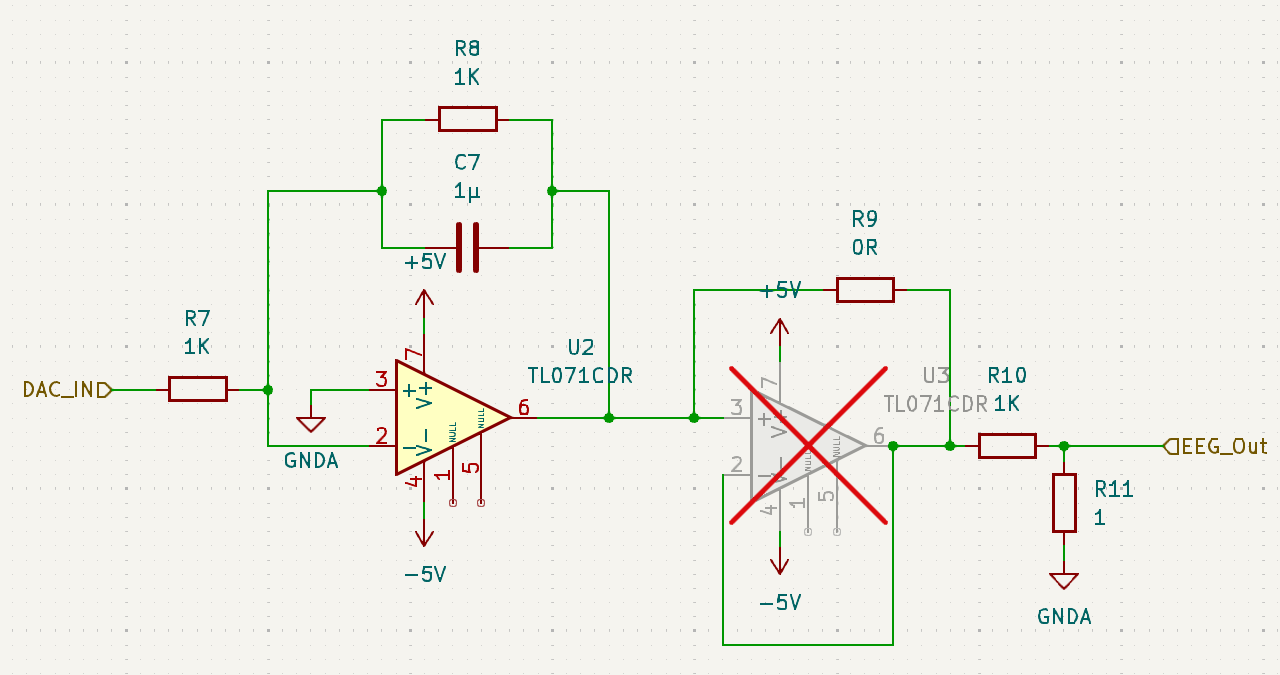
\includegraphics[width=0.8\textwidth]{bilder/Operationsverstaerker_Block.png}
    \caption{Operationsverstärker-Block der Platine}
    \label{fig:operationsverstaerker_block}
\end{figure}

Der Operationsverstärker-Block dient der analogen Nachbearbeitung der vom \gls{dac} bereitgestellten Ausgangssignale. Zum Einsatz kommt der TL071CDR, ein rauschoptimierter Operationsverstärker, der in dieser Anwendung als aktiver Tiefpassfilter erster Ordnung konfiguriert ist. Die Hauptfunktion besteht in der Glättung der Signale und der Unterdrückung hochfrequenter Störanteile.
Die Verstärkung des Filters ist auf 1 eingestellt, um die Signalform nicht zu verändern und gleichzeitig die Spannungsausgabe im gewünschten Millivolt-Bereich zu halten.
Optional kann ein zusätzlicher Operationsverstärker bestückt werden, der als Spannungsfolger (Buffer) wirkt. Dieser dient zur Reduzierung der Ausgangsimpedanz und kann insbesondere bei empfindlichen Messeingängen oder längeren Leitungswegen zur Verbesserung der Signalqualität beitragen. In der Standardkonfiguration ist dieser Pfad durch einen Jumper überbrückt und nicht bestückt.


\subsection{Spannungsversorgung}
\begin{figure}[H]
    \centering
    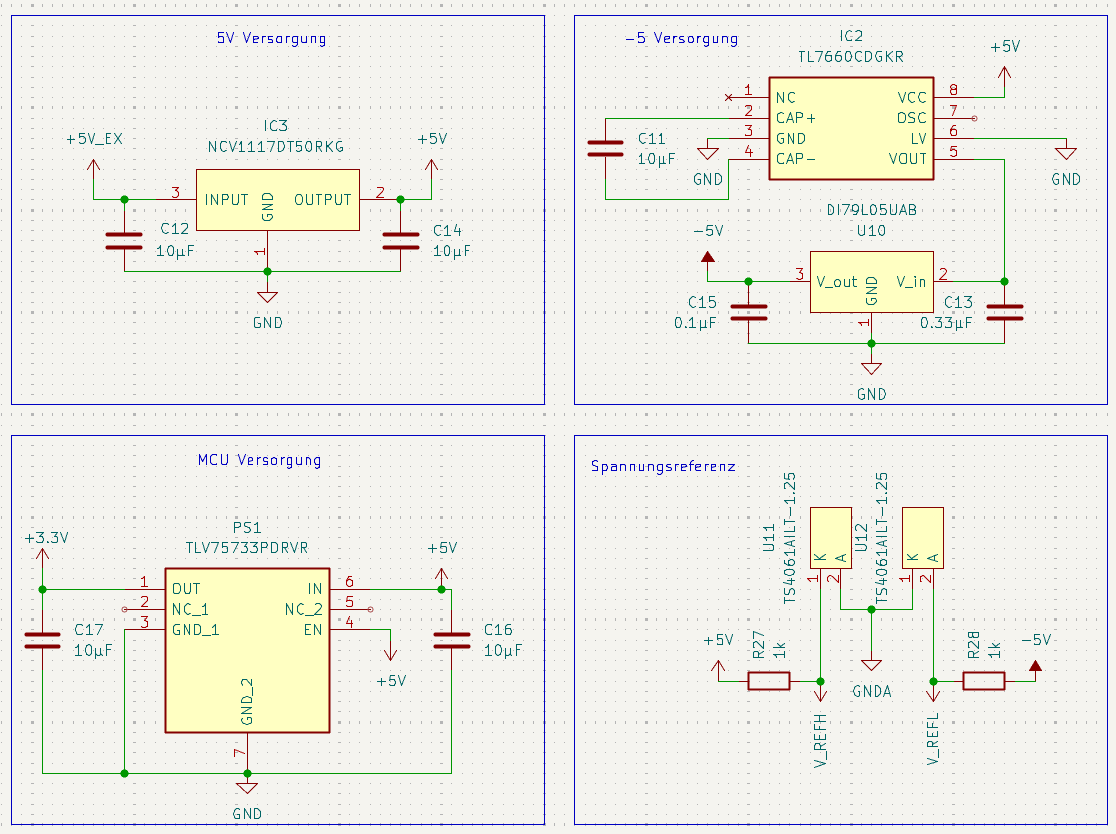
\includegraphics[width=0.8\textwidth]{bilder/Bipolar_Power.png}
    \caption{Spannungsversorgungsblock der Platine}
    \label{fig:spannungsversorgung}
\end{figure}

Die Spannungsversorgung der Platine erfolgt primär über eine USB-Schnittstelle, die eine Eingangsspannung von 5\,V bereitstellt. Diese Spannung wird durch den Linearregler NCV1117DT50RKG stabilisiert und zur Versorgung des DACs sowie der analogen Ausgangsstufen verwendet.
Für die Versorgung des Mikrocontrollers steht ein separater Low-Dropout-Regler (TLV75733PDRVR) zur Verfügung, der die benötigten 3{,}3\,V bereitstellt.
Da der \gls{dac} DAC8412FPZ eine symmetrische Versorgung von $\pm$5\,V erfordert, wird zusätzlich ein invertierender DC/DC-Wandler (LT3580EDD) eingesetzt. Dieser erzeugt aus der 5\,V-Versorgungsspannung eine negative Spannung von –5\,V, die ebenfalls zur Versorgung der Operationsverstärker verwendet wird.
Zudem benötigt der \gls{dac} eine präzise Referenzspannung. Diese wird über zwei Shunt-Referenzbausteine vom Typ TS4061AILT-1.25 realisiert und stellt eine stabile $\pm$1{,}25\,V-Referenz zur Verfügung. Diese Referenz ist entscheidend für die Genauigkeit der analogen Ausgangssignale.

\subsection{USB-Block}
\begin{figure}[H]
    \centering
    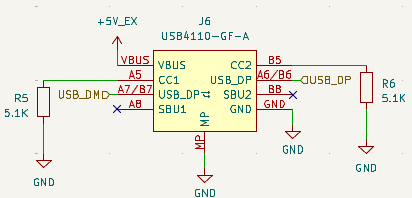
\includegraphics[width=0.8\textwidth]{bilder/USBC_Port.png}
    \caption{USB-Block der Platine}
    \label{fig:usb_block}
\end{figure}

Der USB-Block bildet die primäre Schnittstelle zur Stromversorgung der Platine. Über einen USB-C-Anschluss wird eine standardisierte 5\,V-Spannung bereitgestellt, die anschließend im Spannungsversorgungsblock weiter aufbereitet wird. Zusätzlich enthält der Block grundlegende Schutz- und Filterelemente zur Absicherung der Versorgungsspannung gegen Spannungsspitzen und Verpolung.
Optional kann die USB-Schnittstelle auch zur Datenübertragung mit dem Mikrocontroller verwendet werden, beispielsweise während der Programmierung oder zum Debugging über die serielle Schnittstelle. In der typischen Anwendung wird die Kommunikation jedoch vollständig über die WLAN-Funktion des ESP32 abgewickelt.

\section{Layout und PCB-Design}

\begin{figure}[H]
    \centering
    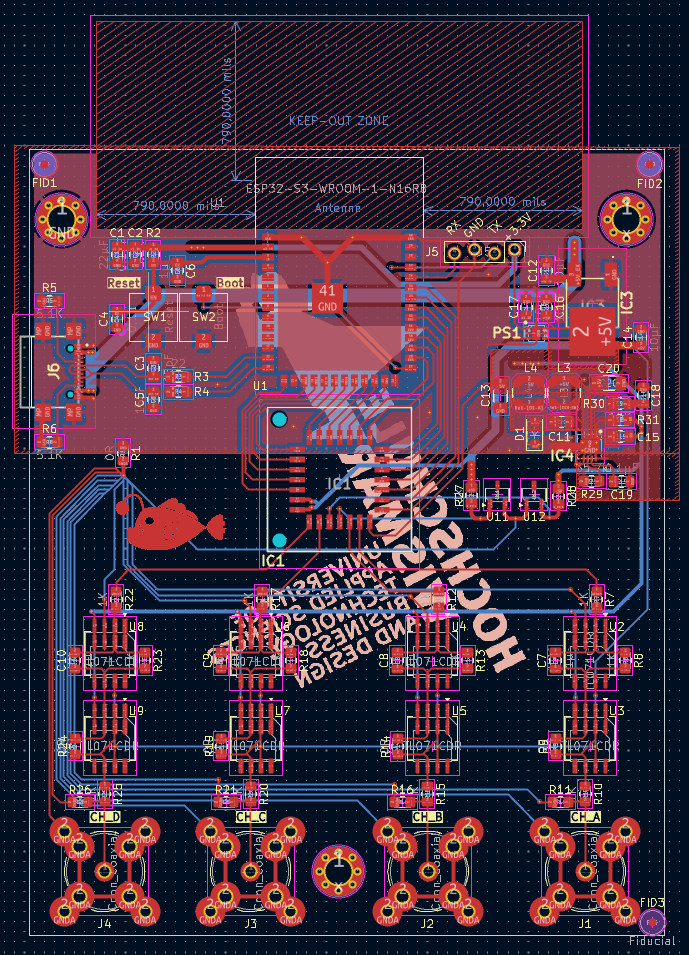
\includegraphics[width=0.8\textwidth]{bilder/Platinen-Layout.png}
    \caption{Layout der Platine}
    \label{fig:usb_block}
\end{figure}

Das PCB-Design wurde mit Fokus auf klare Signalführung, minimale Störanfälligkeit und eine strukturierte Blocktrennung umgesetzt. Die zweilagige Leiterplatte gliedert sich logisch in funktionale Bereiche, wobei sowohl die digitale Steuerung als auch die analogen Ausgangspfade übersichtlich und EMV-gerecht angeordnet sind.
Der Mikrocontroller (ESP32-S3) befindet sich im oberen Bereich der Platine und kommuniziert über eine parallele Busanbindung mit dem darunter angeordneten DAC8412FPZ. Die digitalen Steuersignale sind dabei als kurze, breit geführte Leitungen ausgeführt, um Reflexionen und Timing-Probleme zu minimieren.
Die vier analogen Ausgangskanäle befinden sich im unteren Bereich der Platine. Jeder Kanal verfügt über eine eigene Tiefpassfilterstufe sowie individuell geführte Ausgänge, die über identisch dimensionierte Leitungen auf korrekte Impedanz und Symmetrie geachtet wurden.
Die Versorgungsspannungen verlaufen sternförmig von der zentralen Spannungsaufbereitung aus, wobei Filterkondensatoren lokal an jedem Block platziert sind. Besonders im Bereich der symmetrischen Versorgung (±5\,V) und der Referenzspannungen wurde auf kurze Wege, Masseführung und Potentialtrennung geachtet.
Zudem wurde eine definierte „Keep-Out-Zone“ um die Antenne des ESP32 ausgewiesen, um Störungen im WLAN-Bereich zu vermeiden.